\documentclass[
	12pt,				% tamanho da fonte
	openright,			% capítulos começam em pág ímpar (insere página vazia caso preciso)
	oneside,			
	a4paper,			% tamanho do papel
	chapter=TITLE,		% títulos de capítulos convertidos em letras maiúsculas
	section=TITLE,		% títulos de seções convertidos em letras maiúsculas
	%subsection=TITLE,	% títulos de subseções convertidos em letras maiúsculas
	%subsubsection=TITLE,% títulos de subsubseções convertidos em letras maiúsculas
	% -- opções do pacote babel --
	english,			% idioma adicional para hifenização
	brazil,				% o último idioma é o principal do documento
	]{abntex2}

\usepackage{udesc}

\usepackage{float} % para forçar a posição das figuras

% Para fazer marcações:
\usepackage{color}
\usepackage{ulem}
\newcommand\hl{\bgroup\markoverwith
  {\textcolor{yellow}{\rule[-.5ex]{2pt}{2.5ex}}}\ULon}

% Para desenhar (autômatos, e.g.):
\usepackage{tikz}
\usetikzlibrary{automata, positioning, arrows}
\tikzset{
    node distance=3cm,
    every state/.style={semithick},
    double distance=2pt,
    every edge/.style={
        draw,
        ->,>=stealth',
        auto,
        semithick
    },
    initial text=$ $
}

\usepackage{amsmath}

\usepackage{amssymb} % para usar o símbolo de conjunto vazio

% Para determinar o número da última página na Ficha Catalográfica:
\usepackage{lastpage}

% Para agilizar a inserção de figuras:
\newcommand{\figura}[4]{
	\begin{figure}[H]
    	\caption{#1}
    	\begin{center}
        	#2
    	\end{center}
    	\legend{Fonte: #4.}
    	\label{#3}
    \end{figure}
}
\newcommand{\figuradoautor}[3]{
    \figura{#1}{#2}{#3}{Elaborada pelo autor, 2019}
}

% Dados da capa:
\titulo{Especificação e prova de propriedade acerca de autômatos finitos determinísticos assistidas por Coq}
\autor{Filipe Ramos}
\local{Joinville - SC}
\instituicao{Universidade do Estado de Santa Catarina - Udesc}
\campus{Centro de Ciências Tecnológicas - CCT}
\curso{Bacharelado em Ciência da Computação}
\data{2019}
\fulldata{xx de xxxx de 2019}

% Dados da folha de rosto:
\inforosto{Trabalho de Conclusão de Curso apresentado ao curso de Bacharelado em Ciência da Computação como requisito parcial para a obtenção do título de Bacharel em Ciência da Computação.}
\orientador{Karina Girardi Roggia}
\orientadorRotulo{Dra. }
\coorientador{Rafael Castro Gonçalves Silva}
\coorientadorRotulo{Me. }

\begin{document}

%!TEX root = ../Principal.tex
% Capa do trabalho
\imprimircapa


% Folha de rosto
%* indica que tem ficha catalográfica
\imprimirfolhaderosto*


% Caso a Biblioteca da UDESC forneça, utilize o comando
% \begin{fichacatalografica}
%     \includepdf{fig_ficha_catalografica.pdf}
% \end{fichacatalografica}

% Geração da ficha catalográfica via LaTeX
\begin{fichacatalografica}
	\vspace*{\fill}					% Posição vertical
	\begin{center}					% Minipage Centralizado
	\begin{minipage}[c]{12.5cm}		% Largura
	
	\imprimirautor
	
	\hspace{0.5cm} \imprimirtitulo  / \imprimirautor. --
	\imprimirlocal, \imprimirdata-
	
	\hspace{0.5cm} \pageref{LastPage} p. : il. (algumas color.) ; 30 cm.\\
	
	\hspace{0.5cm} \imprimirorientadorRotulo~\imprimirorientador\\
	
	\hspace{0.5cm}
	\parbox[t]{\textwidth}{\imprimirtipotrabalho~--~\imprimirinstituicao,
	\imprimirdata.}\\
	
	\hspace{0.5cm}
		1. Tópico 01.
		2. Tópico 02.
		I. Prof. Dr. xxxxx.
		II. Universidade do Estado de Santa Catarina.
		III. Centro de Educação do Planalto Norte.
		IV. identificação xxxx\\ 			
	
	\hspace{8.75cm} CDU 02:121:005.7\\
	
	\end{minipage}
	\end{center}
\end{fichacatalografica}


% Folha de aprovação
% Exemplo de folha de aprovação antes da Banca. Após isso, incluia o pdf digitalizado com as assinaturas%
% \includepdf{folhadeaprovacao_final.pdf}
\begin{folhadeaprovacao}

	\begin{center}
		{\ABNTEXchapterfont\bfseries\imprimirautor}
		\vspace{6em}

			\ABNTEXchapterfont\bfseries\imprimirtitulo
		
	\end{center}
		\vspace{1em}
		{\justify
		Trabalho de Conclusão de Curso apresentado ao curso de Bacharelado em Ciência da Computação como requisito parcial para a obtenção do título de Bacharel em Ciência da Computação}
	
	\vspace{3em} 
	\noindent
	{\bfseries Banca examinadora:}
	\assinatura{\textbf{Dra. Karina Girardi Roggia} \\ Instituto Superior Técnico de Lisboa} 
	\assinatura{\textbf{Dr. Cristiano Damiani Vasconcellos} \\ Universidade Federal de Minas Gerais}
    \assinatura{\textbf{Dr. Roberto Silvio Ubertino Rosso Junior} \\ Loughborough University}

    \vspace*{\fill}
    \begin{center}
    	\imprimirlocal,\,\imprimirfulldata
    \end{center}
\end{folhadeaprovacao}


% Dedicatória
\begin{dedicatoria}				
Dedico este trabalho a...  
\end{dedicatoria}


% Agradecimentos
\begin{agradecimentos}
Gostaria de agradecer...

Aqui devem ser colocadas os agradecimentos às pessoas que de alguma forma contribuíram para a realização do trabalho.
\end{agradecimentos}


% Epígrafe
\begin{epigrafe}	
``frase''
\\
\par
autor
\end{epigrafe}


% Resumo em português
\begin{resumo}
 O resumo deve ressaltar o
 objetivo, o método, os resultados e as conclusões do documento. A ordem e a extensão
 destes itens dependem do tipo de resumo (informativo ou indicativo) e do
 tratamento que cada item recebe no documento original. O resumo deve ser
 precedido da referência do documento, com exceção do resumo inserido no
 próprio documento. (\ldots) As palavras-chave devem figurar logo abaixo do
 resumo, antecedidas da expressão Palavras-chave:, separadas entre si por
 ponto e finalizadas também por ponto.

 \vspace{\onelineskip}
    
 \noindent
 \textbf{Palavras-chaves}: latex, abntex e editoração de texto.
\end{resumo}


% Resumo em inglês
\begin{resumo}[Abstract]
 \begin{otherlanguage*}{english}
	Resumo em inglês
   \vspace{\onelineskip}
 
   \noindent 
   \textbf{Key-words}: latex, abntex e text editoration.
 \end{otherlanguage*}
\end{resumo}


% Lista de figuras
\pdfbookmark[0]{\listfigurename}{lof}
\listoffigures*
\cleardoublepage


% Lista de tabelas
\pdfbookmark[0]{\listtablename}{lot}
\listoftables*
\cleardoublepage


% Lista de quadros
\pdfbookmark[0]{\listofquadrosname}{loq}
\listofquadros*
\cleardoublepage
 % texto dos elementos pré-textuais

% Lista de abreviaturas e siglas:
\begin{siglas}
    \acro{AFD}{Autômato finito determinístico}
    \acro{SED}{Sistema a eventos discretos}
    \acro{VANT}{Veículo aéreo não tripulado}
\end{siglas}

% Lista de símbolos:
%\begin{simbolos}
%	\SingleSpacing
%	\item[\%] Porcentagem
%	\item[$D_{ab}$] Distância Euclidiana
%	\item[$O(n)$] Ordem de um algoritmo
%\end{simbolos}

% Sumário:
\pdfbookmark[0]{\contentsname}{toc}
\tableofcontents*
\cleardoublepage

\textual

% Retira o nome do capítulo do header:
\pagestyle{eudesc}
\aliaspagestyle{chapter}{eudesc}


% Texto principal do TCC:
\chapter{Introdução}

Os autômatos são modelos de máquinas abstratas muito importantes para os estudos da computação teórica. Em particular, os autômatos finitos determinísticos (\acs{AFD}s) reconhecem as linguagens regulares, aplicadas na ciência da computação e tecnologia da informação. Sob outra perspectiva, essa classe de autômatos tem sido utilizada para descrever sistemas do mundo hodierno na automação de indústrias e tecnologias, já que o advento dos sistemas a eventos discretos (\acs{SED}s) impôs um novo paradigma, contrário aos sistemas orientados pelo tempo, que são, em geral, muito bem descritos pelos modelos físicos clássicos e modernos.

Sistemas que são orientados a eventos discretos e assíncronos podem ser modelados por formalismos da matemática discreta, entre eles os autômatos determinísticos, as redes de Petri, \textit{timed models} e cadeias de Markov. São exemplos de SEDs vários sistemas de filas, computacionais, de comunicação, manufatura, tráfego, banco de dados, telefonia, etc. Essas classes não são mutuamente exclusivas, no sentido de haver sistemas de filas que são de manufatura, por exemplo. Podemos modelar SEDs com as características dos sistemas de filas a fim de representar plantas industriais, como linhas de produção complexas. Os AFDs, pois, mostram-se como meios eficientes a esse fim, já que permitem análise por meio de formalismos, o que inclui averiguar a satisfação de propriedades.

A demonstração de propriedades a respeito de AFDs pode ser uma tarefa pouco trivial. Por isso, o emprego de assistentes interativos de provas matemáticas é útil a fim de obter demonstrações válidas. Ademais, tais assistentes reúnem meios formais e computacionais que possibilitam a verificação dos passos da demonstração, auferindo rigor. Entre os assistentes de provas, o Coq destaca-se por ter comunidade extensa e qualidades como a construção de tipos dependentes, motivos pelos quais o presente trabalhou optou por empregá-lo.

Os problemas envolvendo filas em processos concorrentes são muito estudados na ciência da computação e dotados de relevância no que tange aos sistemas de produção industrial, onde a falta de sincronização acarreta eventualmente outros problemas. Se um SED é corretamente modelado por AFDs, devemos ser capazes de identificar as eventuais falhas decorrentes da concorrência por recursos distribuídos em filas, justificando o presente estudo.

O objetivo geral deste trabalho de conclusão de curso consiste em provar, mediante o assistente de provas Coq, propriedades sobre sistemas da automação industrial modelados por AFDs. Os objetivos específicos são: \begin{enumerate}
	\item introduzir os principais conceitos relativos aos SEDs;
	\item apresentar a classe de sistemas de filas;
	\item especificar propriedades desejadas para essa classe;
	\item empregar o assistente Coq na prova de teoremas referentes a essas propriedades;
	\item demonstrar e explanar tais teoremas e exemplificar suas aplicações. 
\end{enumerate}

Com a finalidade de atingir os objetivos supracitados, o presente trabalho é estruturados destarte. Primeiramente, apresenta-se uma breve noção sobre assistentes de provas e elencam-se os artifícios do Coq mais importantes para o trabalho. No capítulo \ref{cap:seds}, são introduzidos os SEDs, assim como sua modelagem por AFDs. O capítulo seguinte, \ref{cap:filas}, apresenta os sistemas de filas, problemas relacionados e as propriedades mais importantes acerca desses SEDs. Em seguida, o capítulo \ref{cap:propriedades} demonstra como constatar se sistemas de filas atendem às propriedades. Por fim, são expressas as considerações finais e, depois, as referências bibliográficas.
\chapter{Assistentes de provas}

Um assistente de provas interativo é um artifício de software que auxilia no processo de provas matemáticas ...

\section{Teoria dos tipos}

\section{Coq}

\cite{chlipala}
\chapter{Sistemas a eventos discretos}
\label{cap:seds}

\section{Controle supervisório}

\section{Autômatos finitos determinísticos}

No âmbito dos SEDs, um autômato finito determinístico (AFD) é uma máquina abstrata cujo funcionamento é descrito por uma dada carga de trabalho ordenada sequencialmente. Ao processar a informação de entrada, codificação sobre as operações requisitadas, o AFD acarreta duas possíveis circunstâncias: a operação corrente não é possível no estado atual da máquina -- e portanto o funcionamento é abortado -- ou toda operação é possível e feita. Nos dois casos, ao término, o estado do AFD é reiniciado. Além disso o único efeito interno das operações é a transição de estado, a quantidade de estados em que a máquina pode transitar é finita -- motivo pelo qual ela é denominada outrossim -- e ela não pode estar em mais de um estado simultaneamente, razão por que é determinística. O fato de os eventos, ou operações, ocorrerem em tempo discreto justifica sua modelagem nas teorias dos SEDs. O comportamento de vários desses sistemas pode ser modelado de forma simples, com AFDs.

Alguns estados dos AFDs podem ser marcados para algumas finalidades. Essas máquinas podem proporcionar formalismos reconhecedores de strings; é por isso que às vezes se refere às sequências de operações como palavras.

\subsection{Definição formal segundo \citeonline{hopcroft}}

Haja vista que o presente trabalho objetiva especificar e demonstrar teoremas a respeito de AFDs, é indispensável definir essa classe de máquinas abstratas mediante formalismo. \citeonline{hopcroft} formulam AFD como uma quíntupla \begin{equation}\label{eq:afd_hopcroft}\langle Q, E, \delta, q_0, Q_m \rangle\end{equation} em que: \begin{itemize}
    \item $Q$ é seu conjunto finito não vazio de estados;
    \item $E$ é seu conjunto finito de eventos;
    \item $\delta : Q \times E \nrightarrow Q$ é a função que descreve as transições de estados;
    \item $q_0 \in Q$ é o estado inicial, a partir do qual a máquina inicia seu trabalho;
    \item $Q_m \subseteq Q$ é o conjunto de estados marcados.
\end{itemize}

A definição proposta por \citeonline{cassandras} inclui uma função de estados ativos $\Gamma : Q \rightarrow 2^E$ relacionando as operações possíveis a partir de um estado.

\subsection{Diagrama de estados}

Para auxiliar na visualização das transições entre os estados dos autômatos, os AFDs são comumente representados por diagramas de estados. Nessa representação, os estados são nós de uma estrutura semelhante a de grafos, e as transições, arestas que interligam dois nós, conforme a Figura \ref{fig:afd_diagrama}. Representam-se as transições cuja origem e destino são o mesmo estado por laços que partem de um nó e terminam no mesmo.

\figuradoautor{Representação da transição no diagrama de estados}{
    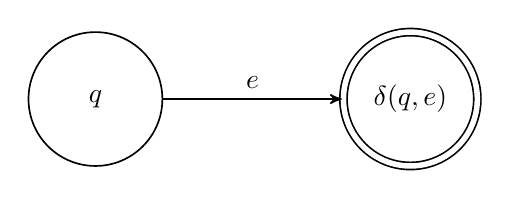
\begin{tikzpicture}
        \node[state,minimum size=1.7cm] (q0) {$q$}; 
        \node[state,accepting,minimum size=1.7cm] at (4,0) (q1) {$\delta(q, e)$};
        \draw
        (q0) edge node{$e$} (q1);
    \end{tikzpicture}
}{fig:afd_diagrama}

Nessa classe de diagramas, os estados inicial e marcados podem ser destacados de alguma forma. Para este trabalho, uma seta sem nó de origem aponta sempre para o nó do estado inicial, e uma circunferência dupla enfatiza o de um estado final, como demonstra a Figura \ref{fig:afd_estado_inicial}.

\figuradoautor{Representação de estados inicial (à esquerda) e marcado (à direita) no diagrama}{
    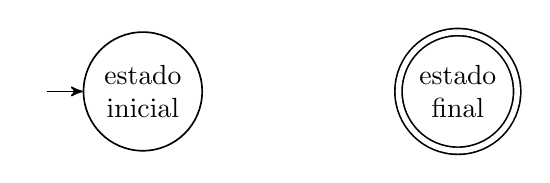
\begin{tikzpicture}
        \node[align=center,state,initial] (q0) {estado\\inicial};
        \node[align=center,state,accepting] at (4,0) (qf) {estado\\final};
    \end{tikzpicture}
}{fig:afd_estado_inicial}

Pode-se citar outros aspectos desta representação de autômatos: a possibilidade de adicionar rótulos aos nós, a opção de omitir os nomes dos estados nos nós quando não forem necessários e a aglutinação de transições que partem e terminam no mesmo estado em uma mesma aresta, com os símbolos separados por vírgula.

\subsection{Linguagens}

\subsection{Função de transição total e estado de ralo}

\subsection{Definição formal para Coq}

Embora amplamente aceitas, as definições matemáticas clássicas de AFD não podem ser diretamente aplicadas no assistente de provas Coq. Ele é, como explana o Capítulo \ref{cap:coq}, uma implementação de teoria de tipos; assim, é necessário que os elementos integrantes da definição tenham tipos. Ademais, implementações de teoria de conjuntos nessa plataforma não são triviais da forma que se apresentam na lógica interpretada por humanos. É incontrovertível deparar-se com a pergunta: como definir AFDs para estes propósitos e de modo correto?

À primeira vista mostra-se factível utilizar tipos indutivos em vez de implementar estruturas de dados para representar conjuntos. Sendo $\{ q_1, q_2, ..., q_k \}$ e $\{ e_1, e_2, ..., e_l \}$ os respectivos conjuntos de estados e eventos de um AFD, pode-se construir
\begin{equation}\text{\mintinline[escapeinside=!!,mathescape]{coq}{
Inductive Q : Type := q1 | q2 | !$...$! | qk.
}}\label{eq:Q_inductive}
\end{equation}
para os estados e
\begin{equation}\text{\mintinline[escapeinside=!!,mathescape]{coq}{
Inductive E : Type := e1 | e2 | !$...$! | el.
}}\label{eq:E_inductive}\end{equation}
para os eventos. Contudo, a fim de representar conjuntos finitos genéricos, essas construções não são possíveis. Representá-los como tipos quaisquer também não é sempre uma alternativa conveniente, já que isso permite instanciar tipos contendo infinitos elementos. A prova da decidibilidade de vários [citar exemplos] problemas acerca de AFDs baseia-se na finitude dos conjuntos de estados e eventos, evidenciando a importância de restringir tal atributo.



[Colocar opções que achei do StackOverflow]

Outra opção tange a especificar o recipiente dos estados na forma de lista e atribuir restrições a ela, fazendo o mesmo para os eventos. A seguinte construção foi adotada:

\begin{minted}[escapeinside=!!]{coq}
Record AFD (A B:Type) : Type := {
  Q : list A;
  E : list B;
  transi!çã!o : A -> B -> A;
  q0 : A;
  Qm : list A;
  ralo : A;
  transi!çã!o_correta : forall q e, transi!çã!o q e <> ralo -> In e E /\ In q Q /\ q <> ralo /\ In (transi!çã!o q e) Q;
  q0_correto : In q0 Q;
  Qm_correto : forall q, In q Qm -> In q Q;
  ralo_correto : In ralo Q
}.
\end{minted}

Restringir a decidibilidade das igualdades de \mintinline{coq}{A} e \mintinline{coq}{B} é importante no sentido de garantir as igualdades decidíveis dos AFDs\footnote{Os conjuntos de estados e eventos são finitos; logo, como aborda a Subseção \ref{ssec:eq_decidivel}, a igualdade entre seus elementos é decidível.} e permitir aplicar a proposição \mintinline[escapeinside=!!]{coq}{transi!çã!o_correta}, pois verificar se, para quaisquer elementos \mintinline{coq}{q:A} e \mintinline{coq}{e:B}, \mintinline[escapeinside=!!]{coq}{transi!çã!o q e} é igual ao estado de ralo requer $$\text{\mintinline{coq}{forall x, {x = ralo} + {x <> ralo}}}$$ Mais, essa restrição facilita a prova de alguns dos lemas demonstrados pelo presente trabalho. Ela pode ser assim adicionada ao \mintinline{coq}{Record AFD}:

\begin{minted}[escapeinside=!!]{coq}
A_decid!í!vel : forall (x y:A), {x = y} + {x <> y};
B_decid!í!vel : forall (x y:B), {x = y} + {x <> y}
\end{minted}

A restrição não impede que qualquer AFD definido de acordo com a Equação \ref{eq:afd_hopcroft} seja escrito nesta formulação, porque os conjuntos de estados e eventos dos AFDs podem ser construídos com os tipos das Equações \ref{eq:Q_inductive} e \ref{eq:E_inductive}, inserindo todos os elementos dessas definições indutivas nas respectivas listas de estados e eventos. A igualdade é decidível para qualquer tipo definido conforme as Equações \ref{eq:Q_inductive} e \ref{eq:E_inductive}. A prova disso é feita por análise de casos da seguinte maneira:

\begin{minted}[escapeinside=!!]{coq}
Lemma Q_decid!í!vel : forall (x y:Q), {x = y} + {x <> y}.
Proof.
  destruct x, y; auto; right; intros; discriminate.
Qed.
\end{minted}

\noindent
cuja complexidade de tempo é $O(k^2)$, uma vez que a proposição é destruída em $k^2$ casos. Semelhantemente a complexidade para o tipo \mintinline{coq}{Inductive E} é $O(l^2)$. Em cada caso a tática \mintinline{coq}{auto} automaticamente prova a igualdade e \mintinline{coq}{right; intros; discriminate} prova a diferença.

\section{Sistemas de filas}

\chapter{Problemas de filas}
\label{cap:filas}

Os sistemas de filas constituem importante classe de sistemas a eventos discretos (\acs{SED}s) em que entidades ou objetos devem esperar para obter um determinado recurso. Há três elementos básicos que compõem esses sistemas: \begin{itemize}
	\item consumidor: entidade que espera por um recurso;
	\item servidor: o recurso que é aguardado;
	\item fila: o espaço em que os consumidores esperam.
\end{itemize} Os recursos são genericamente denominados servidores por geralmente proverem serviço \cite{cassandras}. O presente trabalho aborda uma ótica abstrata dos sistemas de filas, já que há a possibilidade de reduzir problemas a estes sistemas.

Para ser atendido por um servidor de banco, uma pessoa deve esperar em uma fila até que as pessoas a sua frente sejam atendidas. Esse sistema de filas pode ser modelado pelo autômato infinito determinístico ilustrado pela Figura \ref{fig:fila_simples_infinito}, em que $+$ e $-$ são os respectivos eventos de chegada e partida de pessoa da fila.

\figura{Um sistema de filas simples}{
	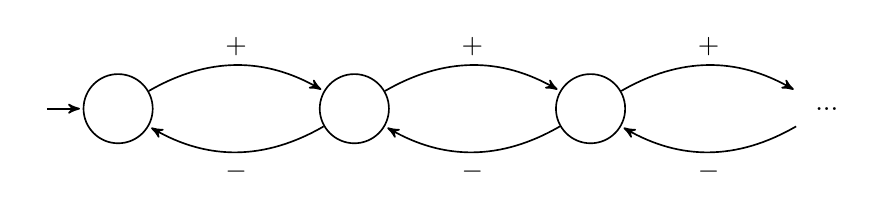
\begin{tikzpicture}[shorten >=1pt,node distance=2cm,on grid,auto] 
		\node[state,initial] (q0) {}; 
		\node[state] at (3,0) (q1) {};
		\node[state] at (6,0) (q2) {};
		\node[state,draw=none] at (9,0) (q3) {$...$};
		\draw
		(q0) edge[bend left, above] node{$+$} (q1)
		(q1) edge[bend left, below] node{$-$} (q0)
		(q1) edge[bend left, above] node{$+$} (q2)
		(q2) edge[bend left, below] node{$-$} (q1)
		(q2) edge[bend left, above] node{$+$} (q3)
		(q3) edge[bend left, below] node{$-$} (q2);
	\end{tikzpicture}
}{fig:fila_simples_infinito}{CASSANDRAS; LAFORTUNE, 1999}

Na Figura \ref{fig:fila_simples_infinito} é assumido que a fila de pessoas pode crescer indefinidamente, o que não é possível na realidade. Assumindo que as filas têm um tamanho máximo, faz-se possível modelar os sistemas de filas por meio de autômatos finitos determinísticos (AFDs). Para muitos destes sistemas, além do mais, deseja-se que as filas respeitem uma capacidade máxima, sem que operações de adição sejam permitidas quando ela é alcançada. Outra propriedade frequentemente esperada é a de que nenhum evento de retirada seja possível quando há zero elementos na fila. A garantia de tais restrições é o que configura o problema do produtor-consumidor \cite{mehmood}, mas não se restringe a ele.

Um exemplo de sistema de filas é apresentado por \citeonline{victor} e consiste em uma planta de fila de demandas para veículos aéreos não tripulados (\acs{VANT}s). Nele as demandas são os consumidores, e os VANTs, os servidores. Seja o AFD da Figura \ref{fig:demandas_vants}, em que os eventos $+$, $a$ e $-$ indicam a chegada, atribuição e conclusão de demanda. O modelo representa um sistema de fila de demandas para VANTs, cujas atribuições só podem ser retiradas da fila depois de concluídas e o tamanho da fila é no máximo $2$. O AFD torna-se complexo se consideramos a possibilidade de falhas e reatribuição, e determinar se restrições são atendidas fica ainda mais difícil.

\figuradoautor{Um sistema de demandas para VANTs}{
	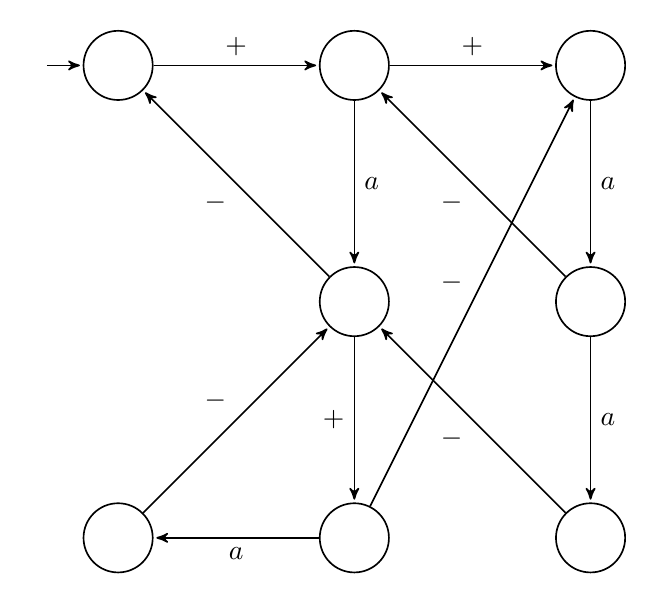
\begin{tikzpicture}[shorten >=1pt,node distance=2cm,on grid,auto]
	\node[state,initial] (q0) {};
	\node[state] at (3, 0) (q1) {};
	\node[state] at (3, -3) (q2) {};
	\node[state] at (3, -6) (q3) {};
	\node[state] at (0, -6) (q4) {};
	\node[state] at (6, 0) (q5) {};
	\node[state] at (6, -3) (q6) {};
	\node[state] at (6, -6) (q7) {};
	\draw
	(q0) edge node{$+$} (q1)
	(q1) edge node{$+$} (q5)
	(q1) edge node{$a$} (q2)
	(q2) edge node{$-$} (q0)
	(q2) edge[left] node{$+$} (q3)
	(q3) edge node{$a$} (q4)
	(q4) edge node{$-$} (q2)
	(q3) edge node{$-$} (q5)
	(q5) edge node{$a$} (q6)
	(q6) edge node{$-$} (q1)
	(q6) edge node{$a$} (q7)
	(q7) edge node{$-$} (q2);
	\end{tikzpicture}
}{fig:demandas_vants} 

A julgar pela dificuldade de garantir consistências em SEDs, é eminente a relevância de métodos formais para inferências a respeito de propriedades dos AFDs. Antes de formular esses meios matemáticos, duas importantes propriedades dos sistemas de filas são expostas na próxima seção, \ref{sec:props}.

\section{Propriedades desejadas}
\label{sec:props}

Como citado para o problema do produtor-consumidor, um sistema de filas geralmente requer que duas propriedades inerentes sejam satisfeitas: que o tamanho máximo de cada fila não possa exceder uma capacidade máxima e não seja possível realizar operações de retirada em uma fila vazia. Isso decorre do fato de que normalmente as filas destes sistemas são representações de espaços físicos, com limitações que devem ser respeitadas nos modelos de SEDs.

O problema do produtor-consumidor decorre da necessidade de sincronizar um \textit{buffer} -- uma fila -- compartilhado entre processos. Na ciência da computação, a concorrência de processos sobre os mesmos recursos impõe que alguns artifícios de software e hardware sejam empregados a fim de respeitar as propriedades explanadas por esta seção. Sem eles, o desenvolvimento de aplicações computacionais com memória compartilhada gera defeitos que são manifestados no uso. Um exemplo deste problema é o caso em que dois processos tentam adicionar arquivo no \textit{spool} de impressão de um sistema operacional, o que, se não for sincronizado, possibilita a ambos os processos escreverem sobre a mesma célula do \textit{spool} \cite{tanenbaum}. No contexto da automação industrial, há também a necessidade de manter processos de produção e manufatura sincronizados. Máquinas que compartilham filas de recursos precisam atuar de modo consistente. 

Apesar de as representações de filas físicas requererem um volume mínimo de zero itens, esta pode não ser uma condição para filas abstratas. A subseção a seguir aborda esses e outros casos, em que é possível reduzir problemas abstraindo a noção de filas, servidores e consumidores.

\subsection{Redução de problemas}

É possível reduzir problemas à validação das propriedades supracitadas. Seja um SED com a seguinte restrição: há dois subconjuntos de eventos $E_1$ e $E_2$ tais que, em qualquer cadeia de eventos executada pelo sistema, o número de elementos pertencentes a $E_1$ menos o número de elementos pertencentes a $E_2$ deve ser menor ou igual a $n$. Abstraindo, podemos imaginar que um supervisor anota um símbolo em uma fila toda vez que um evento de $E_1$ é executado e apaga dela um símbolo quando um evento de $E_2$ é efetuado, da forma que a Figura \ref{fig:reducao_fila} ilustra. Pode-se modelar esse SED como um sistema de filas em que os eventos de $E_1$ e $E_2$ sejam substituídos respectivamente por operações de adição e retirada de fila. Garantido que a fila tem capacidade máxima de $n$ itens, a restrição é satisfeita, porque, sempre que há $x$ símbolos na fila, foram executados $x$ eventos de $E_1$ a mais que de $E_2$.

\figuradoautor{Abstração de filas para redução de problemas}{
	\includegraphics[width=.4 \textwidth]{figuras/reducao_fila.jpg}
}{fig:reducao_fila}

Há outros meios de reduzir problemas de SEDs à garantia das propriedades de sistemas de filas. Para tanto, deve-se encontrar meios de abstraí-los usando os conceitos que este capítulo apresentou. A exemplo dessas abstrações, seja o autômato da Figura \ref{fig:exemplo_reducao1}, que descreve o funcionamento de uma linha de produção em que há uma esteira e dois robôs com sensores embutidos. Quando uma peça passa pela esteira e chega perto de um dos robôs, o sensor deste detecta a peça e emite sinal para que o robô pegue-a, faça algum trabalho nela e coloque-a em outra esteira. Se o primeiro robô está ocupado, o segundo detectará por seu sensor a peça passando e poderá executar o trabalho. Suponhamos que uma análise criteriosa do sistema foi levantada e originou o AFD ilustrado e identifiquemos os respectivos eventos $s_1$, $s_2$, $t_1$ e $t_2$ como a detecção de peça pelos sensores do primeiro e segundo robô e a execução de trabalho na peça pelo primeiro e segundo robô.

\figuradoautor{Autômato para o funcionamento de uma linha de produção simples}{
	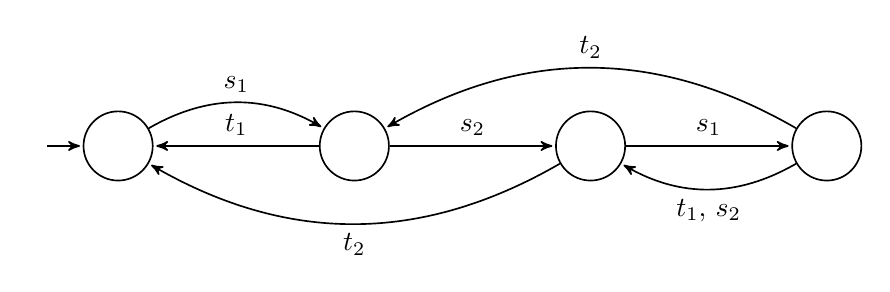
\begin{tikzpicture}[shorten >=1pt,node distance=2cm,on grid,auto] 
	\node[state,initial] (q0) {}; 
	\node[state] at (3,0) (q1) {};
	\node[state] at (6,0) (q2) {};
	\node[state] at (9,0) (q3) {};
	\draw
	(q0) edge[bend left, above] node{$s_1$} (q1)
	(q1) edge[above] node{$t_1$} (q0)
	(q1) edge[above] node{$s_2$} (q2)
	(q2) edge[bend left, below] node{$t_2$} (q0)
	(q2) edge[above] node{$s_1$} (q3)
	(q3) edge[bend left, below] node{$t_1$, $s_2$} (q2)
	(q3) edge[bend right, above] node{$t_2$} (q1);
	\end{tikzpicture}
}{fig:exemplo_reducao1}

Sobre o sistema modelado pela Figura \ref{fig:exemplo_reducao1}, utilizando a abstração por filas, podemos responder à pergunta: há uma carga máxima de trabalho que o segundo robô pode executar a mais que o primeiro? Observando o diagrama, é notável que não. Entretanto, seja uma fila com todos os trabalhos que o segundo robô executa a mais que o primeiro. O sistema de filas da Figura \ref{fig:exemplo_reducao2} apresenta tal redução, e notemos a existência de um ciclo que pode se repetir indefinidas vezes, adicionando um item à fila por vez. Isso evidencia uma característica da fila: não existe capacidade a limitando. O exemplo é simples, mas ilustra claramente uma redução de problema. Para problemas e SEDs complexos, esse procedimento mostra-se interessante, porque propicia o emprego dos métodos matemáticos do presente trabalho na resolução.

\figuradoautor{Autômato da Figura \ref{fig:exemplo_reducao1} reduzido a um sistema de filas}{
	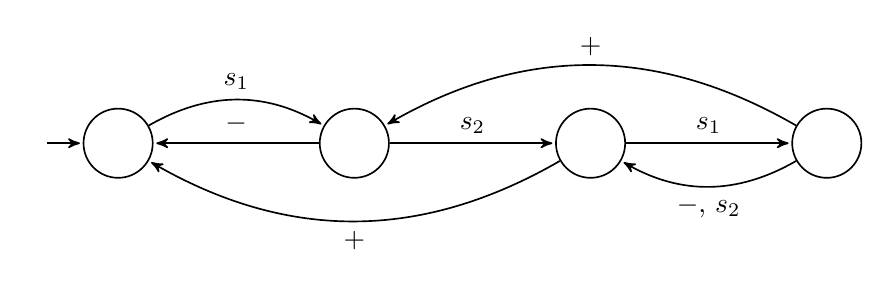
\begin{tikzpicture}[shorten >=1pt,node distance=2cm,on grid,auto] 
	\node[state,initial] (q0) {}; 
	\node[state] at (3,0) (q1) {};
	\node[state] at (6,0) (q2) {};
	\node[state] at (9,0) (q3) {};
	\draw
	(q0) edge[bend left, above] node{$s_1$} (q1)
	(q1) edge[above] node{$-$} (q0)
	(q1) edge[above] node{$s_2$} (q2)
	(q2) edge[bend left, below] node{$+$} (q0)
	(q2) edge[above] node{$s_1$} (q3)
	(q3) edge[bend left, below] node{$-$, $s_2$} (q2)
	(q3) edge[bend right, above] node{$+$} (q1);
	\end{tikzpicture}
}{fig:exemplo_reducao2}

Especificadas as propriedades acima, resta-nos encontrar formalismos capazes de auxiliar a garantia delas. O capítulo seguinte, \ref{cap:propriedades}, propõe e exemplifica teoremas para esse propósito.


\chapter{Considerações parciais}
\label{cap:consideracoes}

Este trabalho apresentou os principais conceitos relacionados à modelagem de sistemas a eventos discretos (\acs{SED}s) por meio de autômatos finitos determinísticos (\acs{AFD}s), bem como os relativos a sistemas de filas. Além disso, foi apresentada a possibilidade de reduzir problemas de SEDs à garantia de propriedades acerca de filas abstratas. Demonstraram-se outras aplicações envolvendo duas restrições de sistemas de filas, que podem ser verificadas por meio de teoremas provados com assistência do Coq. Esse assistente de provas, introduzido no capítulo \ref{cap:provas}, mostrou-se útil no processo de prova interativa, posteriormente transcrita para o relatório.

Os exemplos e aplicações expostos neste relatório evidenciam a relevância de provar a consistência de sistemas com filas, cujas falhas decorrentes do projeto resultam em problemas para a produção automatizada. Também é eminente a utilidade dos formalismos matemáticos na verificação de características esperadas para um sistema. Após o SED ser projetado e modelado, é possível realizar estudos a respeito de seu funcionamento, em que a matemática é artifício de importância.

Alguns teoremas expostos nesta monografia não foram devidamente provados, posto que isso é trabalho futuro. Ainda, novos problemas, aplicações, exemplos, lemas e teoremas podem vir à tona, o que será acrescido ao trabalho final.

% Finaliza o bookmark do PDF:
\bookmarksetup{startatroot}% 

\postextual

% Referências bibliográficas:
\bibliography{referencias}

% Glossário:
%
% Consulte o manual da classe abntex2 para orientações sobre o glossário.
%
%\glossary

% Apêndices:
%\begin{apendicesenv}
%	\include{Partes/apeA}
%\end{apendicesenv}

% Anexos:
%\begin{anexosenv}
%	\include{Partes/aneA}
%\end{anexosenv}

\end{document}

